\pagebreak
\section{Mesh Connectivity [25\%]}
Section 1.7.5 of the notes introduces matrices $\doubleunderline{E}$ and $\doubleunderline{N}$ for describing connections between elements and nodes of a mesh.  Assume that both matrices are made unique by using a counter-clockwise ordering of nodes/elements and by beginning each row with the smallest index.  Element/node numbering starts at 1 and no numbers are skipped.  Assume triangular elements.

\begin{figure}[h]
    \centering
    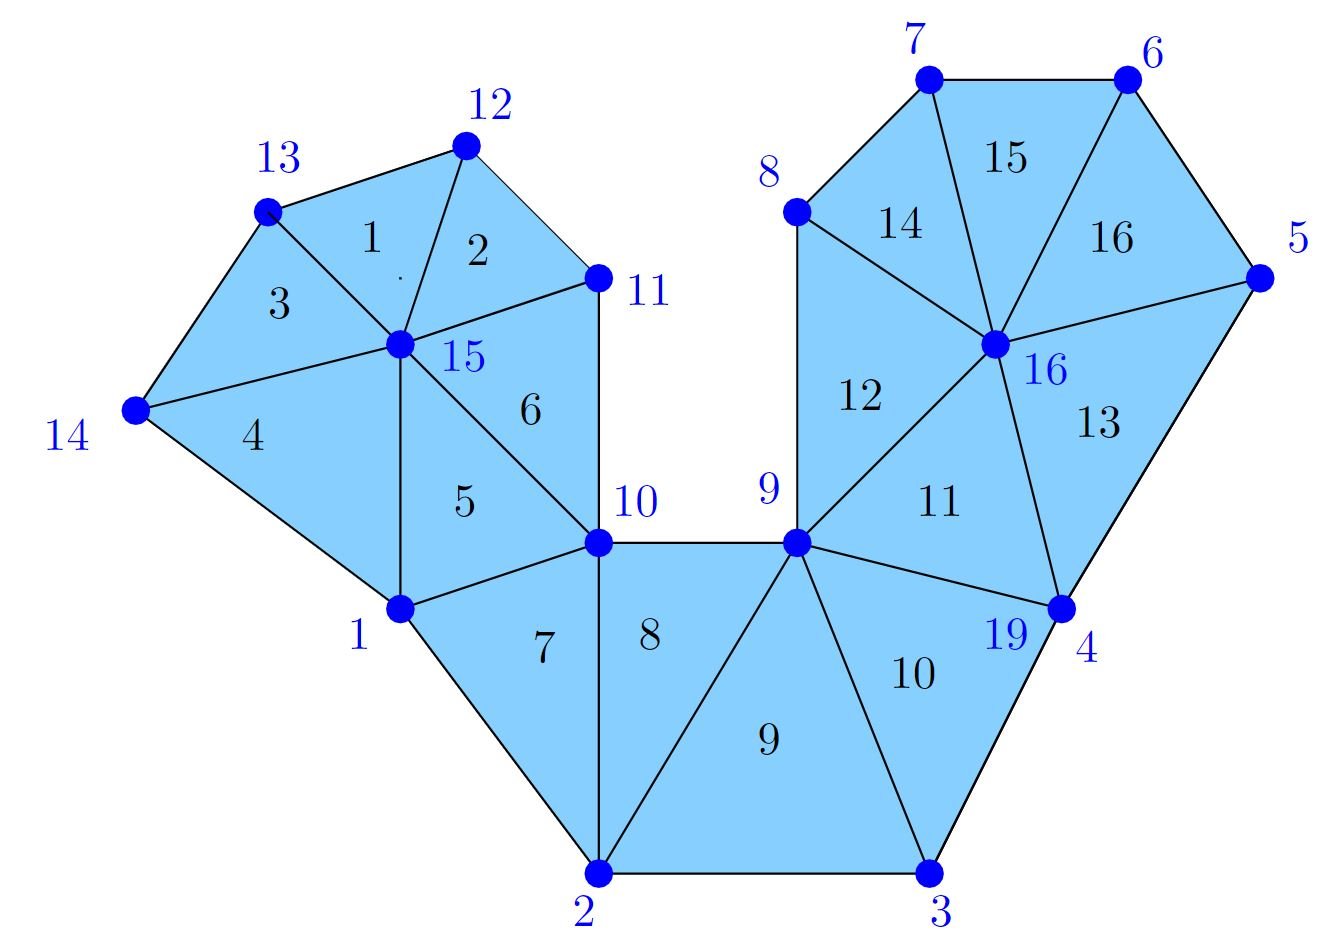
\includegraphics[width = 0.5\linewidth]{q4/q4_diag.JPG}
    \caption{Triangular mesh grid.}
\end{figure}

\begin{enumerate}[label=\alph*., start = 1]
    \item For the mesh shown above, write down the matrices $\doubleunderline{E}$ and $\doubleunderline{N}$.
    
    \begin{equation*}
        \boxed{\doubleunderline{E} = 
        \begin{bmatrix}
            12 & 13 & 15\\  % 1
            11 & 12 & 15\\  % 2
            13 & 14 & 15\\  % 3
            1 & 15 & 14\\   % 4
            1 & 10 & 15\\   % 5
            10 & 11 & 15\\  % 6
            1 & 2 & 10 \\   % 7
            2 & 9 & 10\\    % 8
            2 & 3 & 9\\     % 9
            3 & 4 & 9\\     % 10
            4 & 16 & 9\\    % 11
            8 & 9 & 16\\    % 12
            4 & 5 & 16\\    % 13
            7 & 8 & 16\\    % 14
            6 & 7 & 16\\    % 15
            5 & 6 & 16
        \end{bmatrix},\qquad 
        \doubleunderline{N} = 
        \begin{bmatrix}
            4 & 5 & 7\\ % 1
            7 & 8 & 9\\ % 2
            9 & 10\\    % 3
            10 & 11 & 13\\ %4
            13 & 16\\   % 5
            15 & 16\\   % 6
            14 & 15\\   % 7
            12 & 14\\   % 8
            8 & 9 & 10 & 11 & 12\\  % 9
            5 & 6 & 7 & 8\\         % 10
            2 & 6\\     % 11
            1 & 2\\     % 12
            1 & 3\\     % 13
            3 & 4\\     % 14
            1 & 2 & 3 & 4 & 5 & 6\\ % 15
            11 & 12 & 13 & 14 & 15 & 16\\   % 16
        \end{bmatrix}}
    \end{equation*}
    
    \begin{fminipage}{0.8\linewidth}
        \textbf{Shown above are the matrices for $\bf \doubleunderline{E}$ and $\bf \doubleunderline{N}$ for the irregular mesh as indicated in Section 1.7.5 of the course notes.}
    \end{fminipage}

    \pagebreak
    \item Write a pseudo-code for \underline{efficiently} determining $\doubleunderline{E}$ given $\doubleunderline{N}$. For  this  part,  the  rows  of  the $\doubleunderline{E}$ matrix need not satisfy the ordering requirement.
    
    \textbf{\underline{Pseudo-Code}}
    \begin{enumerate}[label =\arabic*:]
        \item Create $\doubleunderline{E} = [\ ]$
        \item {\tt for i = 1:length($\doubleunderline{N}$)}\quad \textbf{Loop through all the nodes in $\bf \doubleunderline{N}$}
        \item \quad {\tt for j = 1:max(size(N(i,:)))}\quad \textbf{Loop through all the elements for a given node}
        \item \quad\quad E(N(i, j), end) = i \quad \textbf{Place the node value at the end of the the $\bf i$\textsuperscript{th} column in $\bf \doubleunderline{E}$}
        \item \quad end
        \item {\tt end}
    \end{enumerate}

    \begin{fminipage}{0.9\linewidth}
        \textbf{This is the code in theory that should be implemented to be efficiently implemented meaning that it scales $\mathcal{O}({\tt{size}}(\doubleunderline{N}))$. However, placing these values into the $\bf \doubleunderline{E}$ matrix is unique to each given coding programing language (i.e. C++ would use {\tt{.pushback()}}) so in application, with Matlab at least, I would pre-allocate $\bf \doubleunderline{E}$ to be a matrix of {\tt{nan}} and have several {\tt{if, elseif}} statements to determine the ending index for a given iteration {\tt{if}} the last index is {\tt{nan}} and replace with the current node value from the iteration through $\bf \doubleunderline{N}$.}
    \end{fminipage}
    \item How many edges (total, interior and boundary) are in the above mesh?  Write a pseudo-code for \underline{efficiently} determining the number of edges in a mesh given $\doubleunderline{E}$.
    
    \bigskip
    \begin{tabular}{l l}
        \textbf{Total:} & 31\\
        \textbf{Interior:} & 17\\
        \textbf{Boundary:} & 14\\
    \end{tabular}


    \textbf{\underline{Pseudo-Code}}
    \begin{enumerate}[label =\arabic*:]
        \item Create ${\tt \doubleunderline{N}}$ to have empty indices of {\tt nan}
        \item {\tt counter = 0} \quad \textbf{Initialize counter to be zero}
        \item {\tt for j = 1:max(size($\doubleunderline{N}$))}\quad \textbf{Loop through all the nodes}
        \item \quad {\tt for i = 1:max(size($\doubleunderline{N}$(j, :)))}\quad \textbf{Loop through each element adjacent to a node}
        \item \quad\quad {\tt if isnan($\doubleunderline{N}$(j, i)) ~= 1} \quad \textbf{For easy implementation check if value is {\tt nan}, because if so it has been used before and should be skipped}
        \item \quad\quad\quad {\tt [row, col] = find($\doubleunderline{N}$ == $\doubleunderline{N}$(j,i))}\quad \textbf{Find the indices of the node}
        \item \quad\quad\quad {\tt $\doubleunderline{N}$(row(end), col(end)) = nan}\quad \textbf{Replace with {\tt nan} to indicate it's been used}
        \item \quad\quad\quad {\tt counter += 1} \quad \textbf{Increment the counter}
        \item \quad\quad {\tt end if}, {\tt end for(i)}, {\tt end for(j)}
        \item {\tt counter -= 1}\quad \textbf{Since the final pass is ineveitable without heavy modification, increment down after the full pass}
    \end{enumerate}

    \begin{fminipage}{0.9\linewidth}
        \textbf{In the pseudo-code shown above, it scales $\bf \mathcal{O}(N)$ making it as efficient as possible in determining the number of edges. Actual code implementation can be found attached at the end of my assignment.}
    \end{fminipage}
\end{enumerate}


